% !TEX root = ../Tesis.tex
\chapter{Resultados}
\section{Estaciones de monitoreo de calidad de aire}
En la Figura~\ref{fig:ozono} se observa la variación del ozono
(O\textsubscript{3}) durante el periodo de muestreo. La concentración
más alta ocurrió el 23 de febrero con $45$\,ppb en la estación de Cruz
Roja. Por otro lado, el mínimo alcanzado fue en Salamanca con $17$\,ppb
el 20 de febrero.

\begin{figure}[htbp]
    \centering
    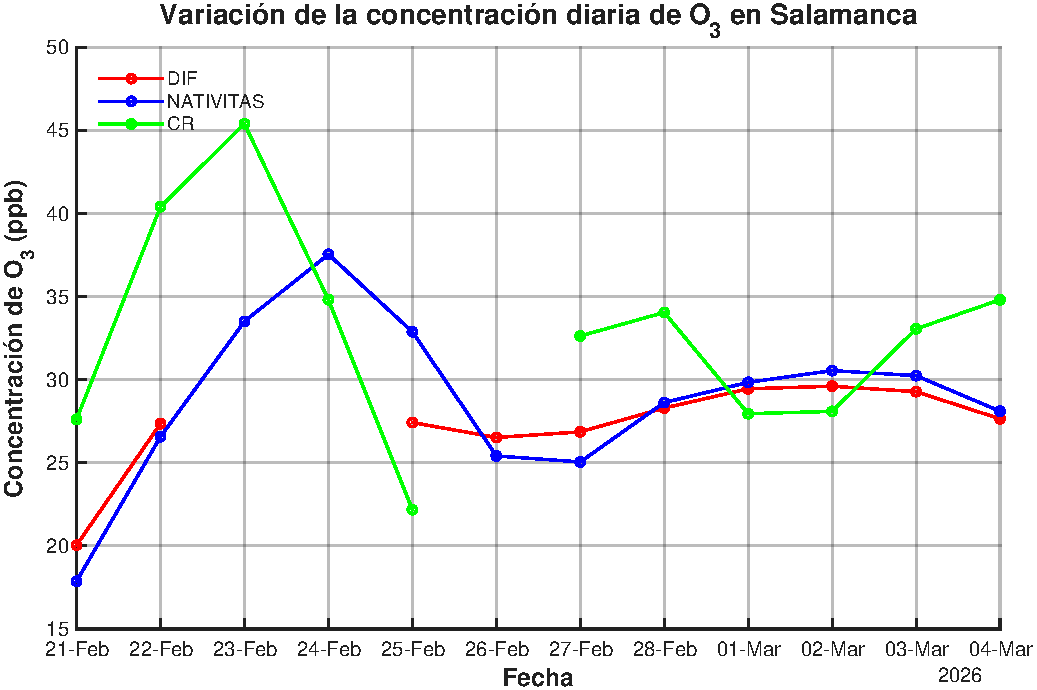
\includegraphics[width=0.85\textwidth]{Resultados/O3_diario.pdf}
    \caption{Variación de la concentración de O\textsubscript{3} en las
    estaciones de monitoreo del del 20 de febrero al 5 de marzo del 2026.}
    \label{fig:ozono}
\end{figure}

En la Figura~\ref{fig:ciclo_ozono} se expone el ciclo diurno del ozono
(O\textsubscript{3}). Se observa que el pico más alto reportado fue a
las 17\,h en la estación DIF y un mínimo a las 7\,h. No existen datos
suficientes para las estaciones de Nativitas y Cruz Roja para obtener un
promedio representativo.

\begin{figure}[htbp]
    \centering
    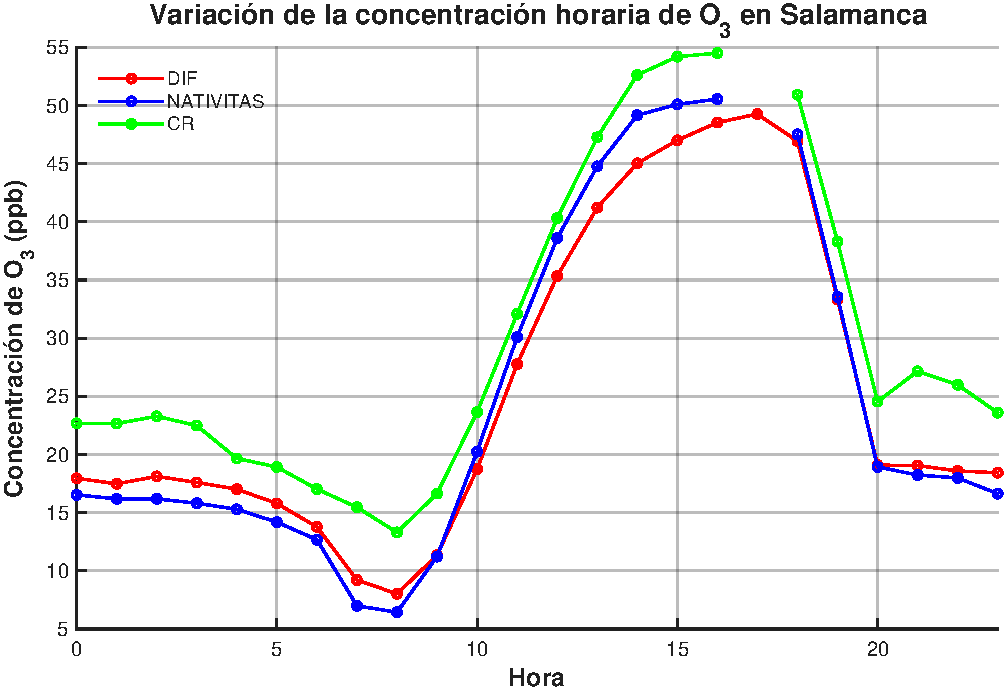
\includegraphics[width=0.85\textwidth]{Resultados/O3_horario.pdf}
    \caption{Ciclo diurno de O\textsubscript{3} del del 20 de febrero al 5 de marzo del 2026}
    \label{fig:ciclo_ozono}
\end{figure}

La variación del dióxido de azufre (SO\textsubscript{2}) se observa en
la Figura~\ref{fig:so2}. La estación de Cruz Roja muestra niveles de
concentración más variables, mientras que Nativitas mantiene
concentraciones superiores a las demás, oscilando entre $18$ y $20$\,ppb.
Por su parte, DIF se mantiene estable, con concentraciones entre $10$ y
$12$\,ppb.

\begin{figure}[htbp]
    \centering
    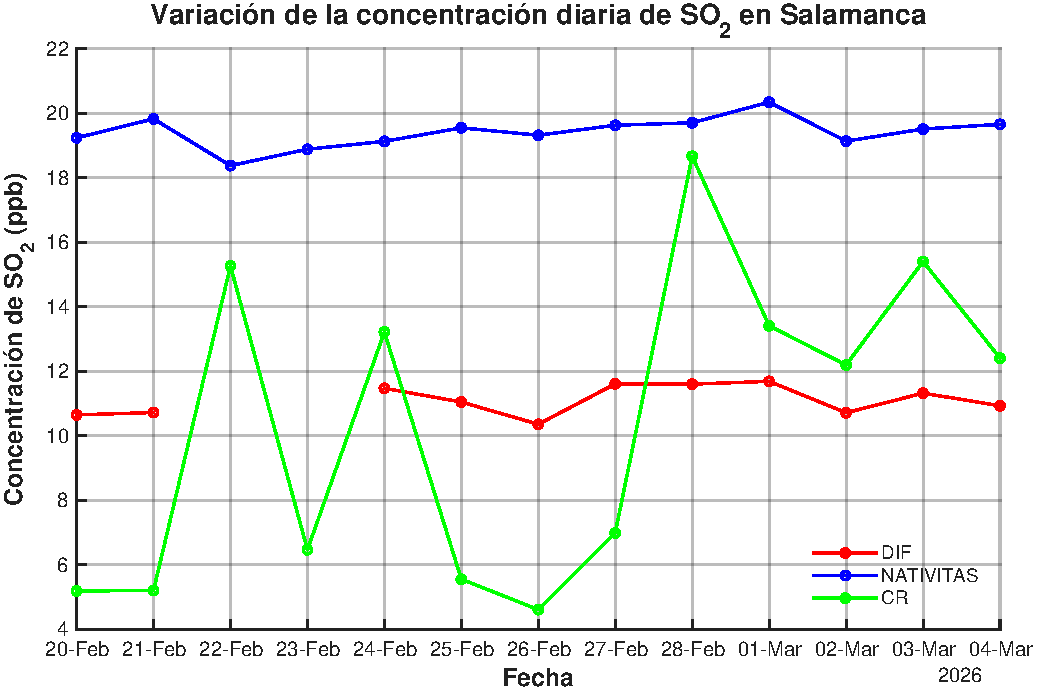
\includegraphics[width=0.85\textwidth]{Resultados/SO2_diario.pdf}
    \caption{Variación de la concentración de SO\textsubscript{2} en las
    estaciones de monitoreo del 20 de febrero al 5 de marzo del 2026.}
    \label{fig:so2}
\end{figure}

Así mismo, la Figura~\ref{fig:so2_horario} refleja la concentración
horaria de dióxido de azufre (SO\textsubscript{2}). El pico más alto de
concentración se presenta en Cruz Roja a las 10\,h y el mínimo a las
18\,h en la misma estación. Mientras tanto, Nativitas y DIF sostienen un
ciclo más estable, con un pico máximo a las 21\,h.

\begin{figure}[htbp]
    \centering
    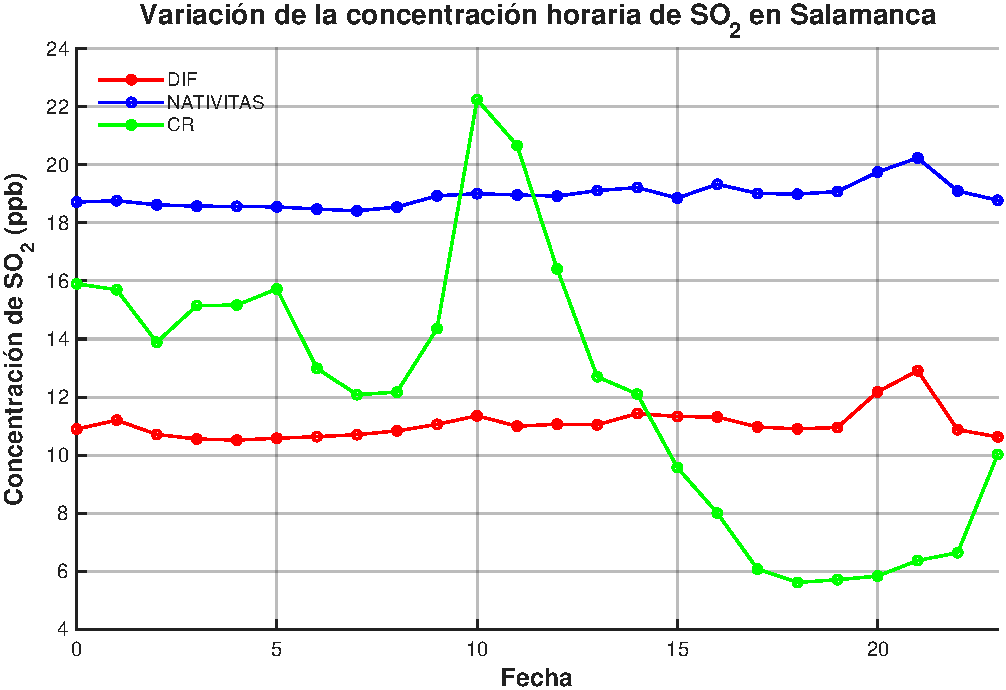
\includegraphics[width=0.85\textwidth]{Resultados/SO2_horario.pdf}
    \caption{Ciclo diurno de SO\textsubscript{2} en las estaciones de
    monitoreo del 20 de febrero al 5 de marzo del 2026.}
    \label{fig:so2_horario}
\end{figure}

Las partículas PM\textsubscript{10} tienen máximos de concentración en
Nativitas, con aproximadamente \SI{100}{\micro\gram\per\cubic\meter} el
22 de febrero. Esta estación presenta las mayores concentraciones,
mientras que DIF presenta el punto mínimo el 2 de marzo con
\SI{45}{\micro\gram\per\cubic\meter} (Figura~\ref{fig:pm10}). Por otro
lado, en el comportamiento horario, Nativitas presenta un pico a las
21\,h y mantiene las máximas concentraciones, excepto en un periodo de
10\,h a 15\,h (Figura~\ref{fig:pm10_horario}).

\begin{figure}[htbp]
    \centering
    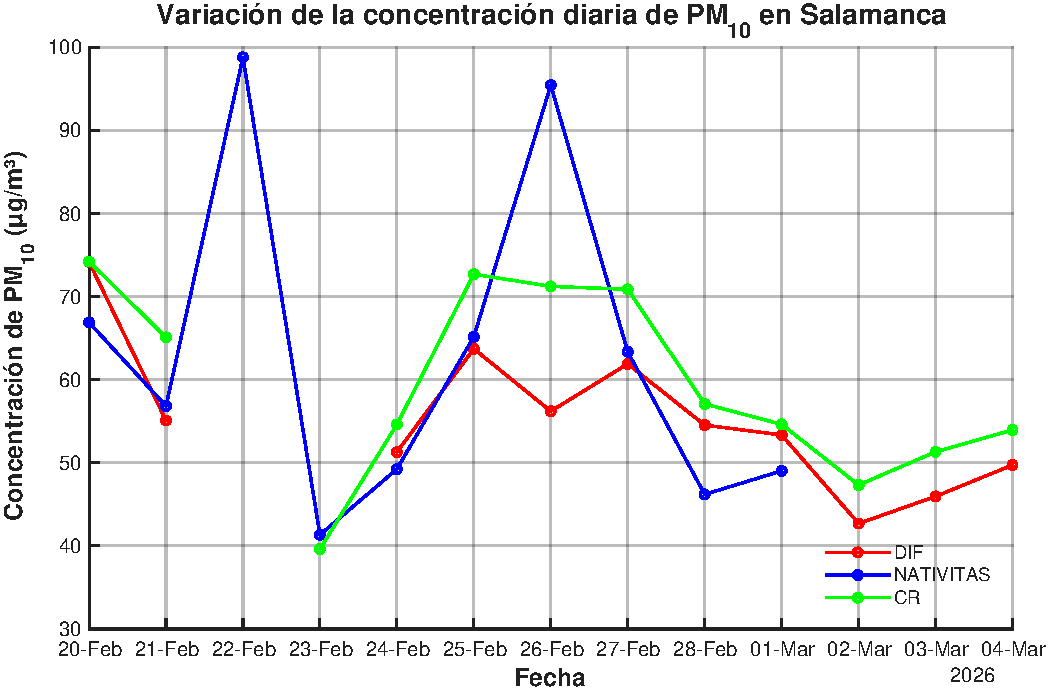
\includegraphics[width=0.85\textwidth]{Resultados/PM10_diario.pdf}
    \caption{Variación de la concentración de PM\textsubscript{10} en las
    estaciones de monitoreo del 20 de febrero al 5 de marzo del 2026.}
    \label{fig:pm10}
\end{figure}

\begin{figure}[htbp]
    \centering
    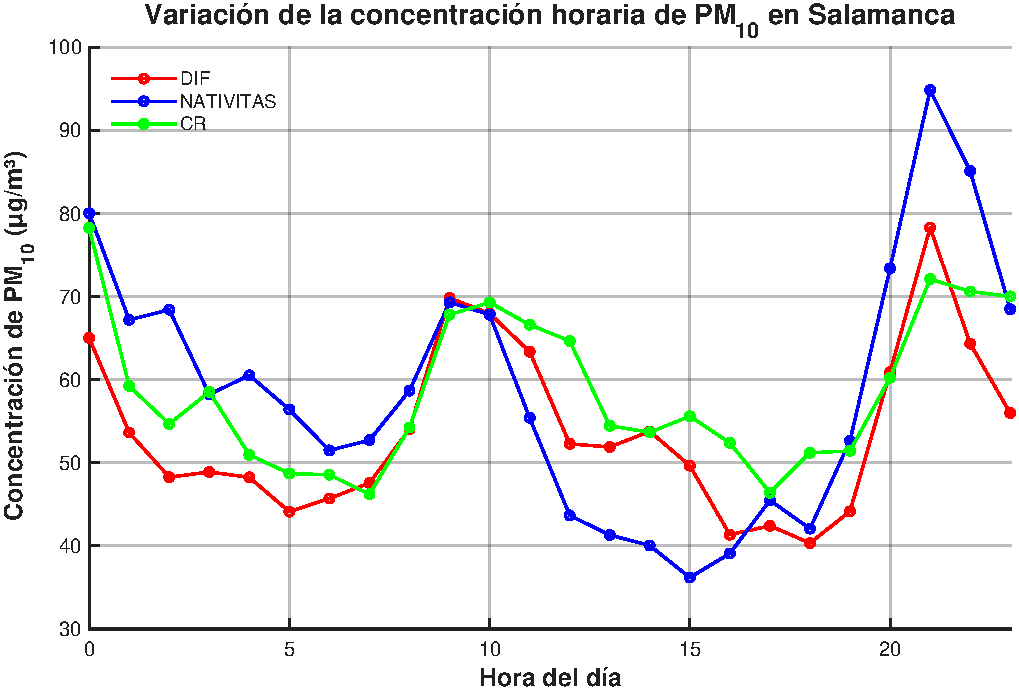
\includegraphics[width=0.85\textwidth]{Resultados/PM10_horario.pdf}
    \caption{Ciclo diurno de PM\textsubscript{10} en las estaciones de
    monitoreo del 20 de febrero al 5 de marzo del 2026.}
    \label{fig:pm10_horario}
\end{figure}

La variación diaria y horaria de PM\textsubscript{2.5} se encuentra en
la Figura~\ref{fig:pm25} y la Figura~\ref{fig:pm25_horario},
respectivamente. Para este contaminante, Nativitas no reporta ninguna
concentración. Por otro lado, DIF presenta las mayores concentraciones,
con un pico máximo el 20 de febrero de aproximadamente
\SI{27}{\micro\gram\per\cubic\meter} y, en el comportamiento horario, a
las 20\,h. Cruz Roja presenta el mínimo el 23 de febrero.

\begin{figure}[htbp]
    \centering
    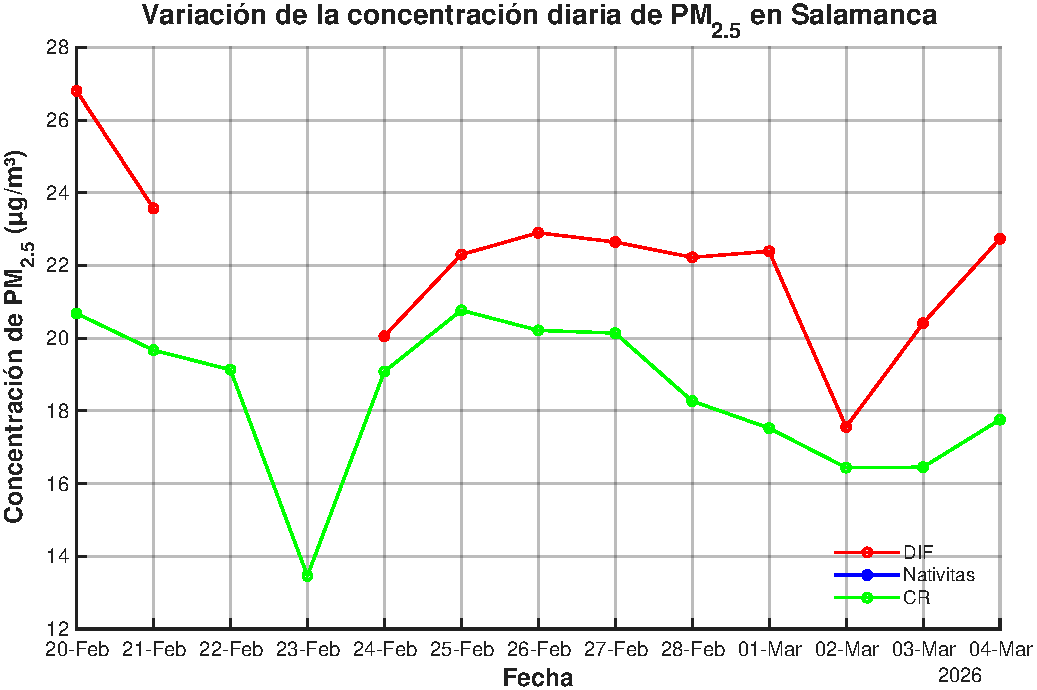
\includegraphics[width=0.85\textwidth]{Resultados/PM25_diario.pdf}
    \caption{Variación de la concentración de PM\textsubscript{2.5} en las
    estaciones de monitoreo del 20 de febrero al 5 de marzo del 2026.}
    \label{fig:pm25}
\end{figure}

\begin{figure}[htbp]
    \centering
    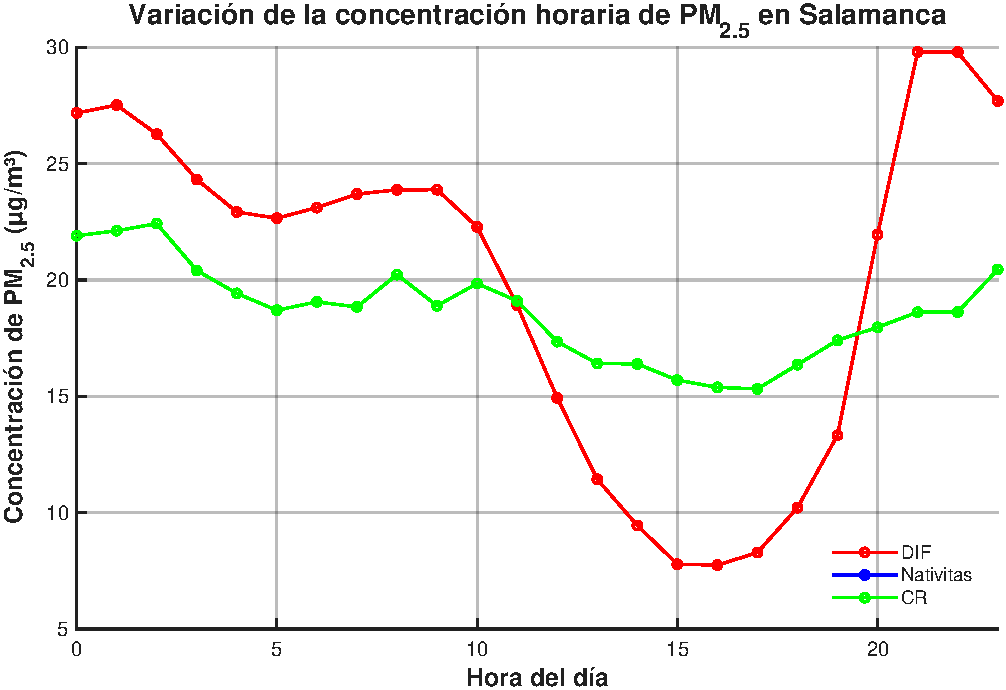
\includegraphics[width=0.85\textwidth]{Resultados/PM25_horario.pdf}
    \caption{Ciclo diurno de PM\textsubscript{2.5} en las estaciones de
    monitoreo del 20 de febrero al 5 de marzo del 2026.}
    \label{fig:pm25_horario}
\end{figure}

La concentración máxima de CO se presenta en Nativitas, con las
máximas concentraciones del 20 al 26 de febrero. Cruz Roja presenta el
mínimo global el 22 de febrero (Figura~\ref{fig:co}). Se observa
ausencia de datos en esta especie. Por otro lado, en el ciclo diurno,
Nativitas conserva las concentraciones más altas, con un pico a las
20\,h. Un segundo pico se presenta a las 8\,h en las tres estaciones
(Figura~\ref{fig:co_horario}).

\begin{figure}[htbp]
    \centering
    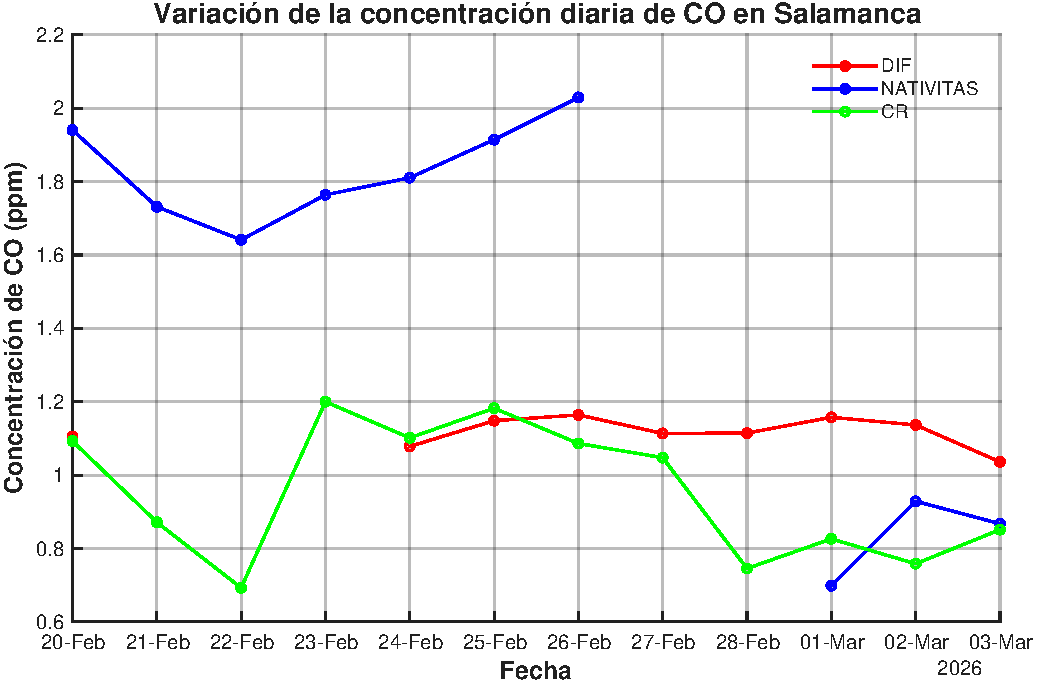
\includegraphics[width=0.85\textwidth]{Resultados/CO_diario.pdf}
    \caption{Variación de la concentración de CO en las estaciones de
    monitoreo durante el periodo de muestreo.}
    \label{fig:co}
\end{figure}

\begin{figure}[htbp]
    \centering
    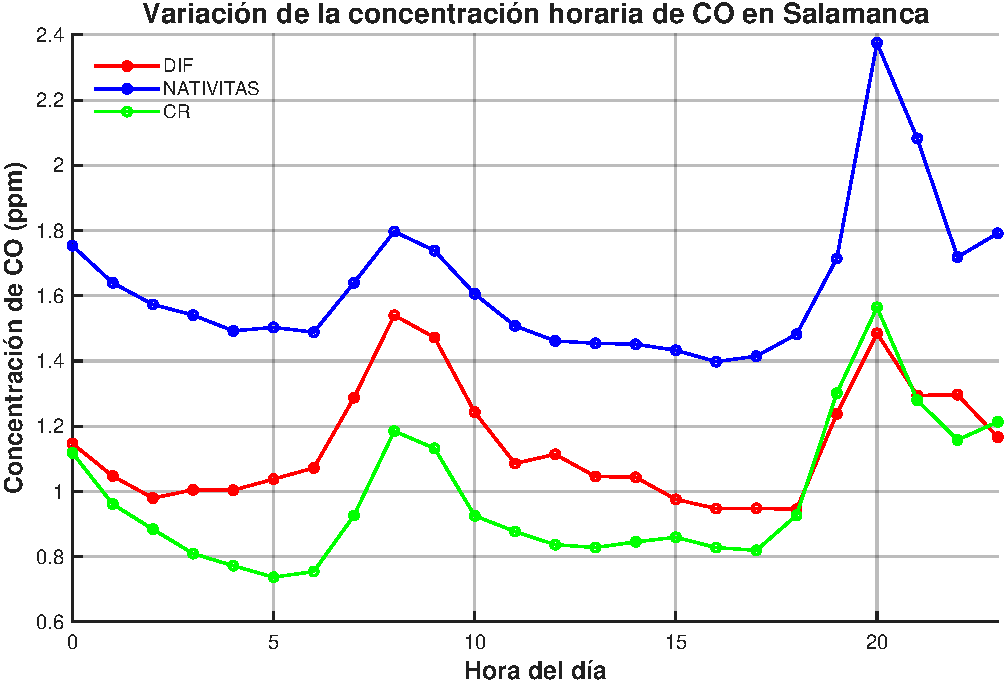
\includegraphics[width=0.85\textwidth]{Resultados/CO_horario.pdf}
    \caption{Ciclo diurno de CO en las estaciones de monitoreo durante
    el periodo de muestreo.}
    \label{fig:co_horario}
\end{figure}

El dióxido de nitrógeno (NO\textsubscript{2}) mantiene concentraciones
superiores en la estación Cruz Roja con respecto a las otras. Los
máximos se encuentran el 27 y 28 de febrero, que conservan
aproximadamente la misma concentración
(\SI{32}{\micro\gram\per\cubic\meter}). En el caso contrario, la
estación DIF mantuvo los niveles más bajos de este contaminante
(Figura~\ref{fig:no2}). En el ciclo diurno se presentan dos picos: el
máximo global a las 20\,h y el segundo a las 8\,h
(Figura~\ref{fig:no2_horario}).

\begin{figure}[htbp]
    \centering
    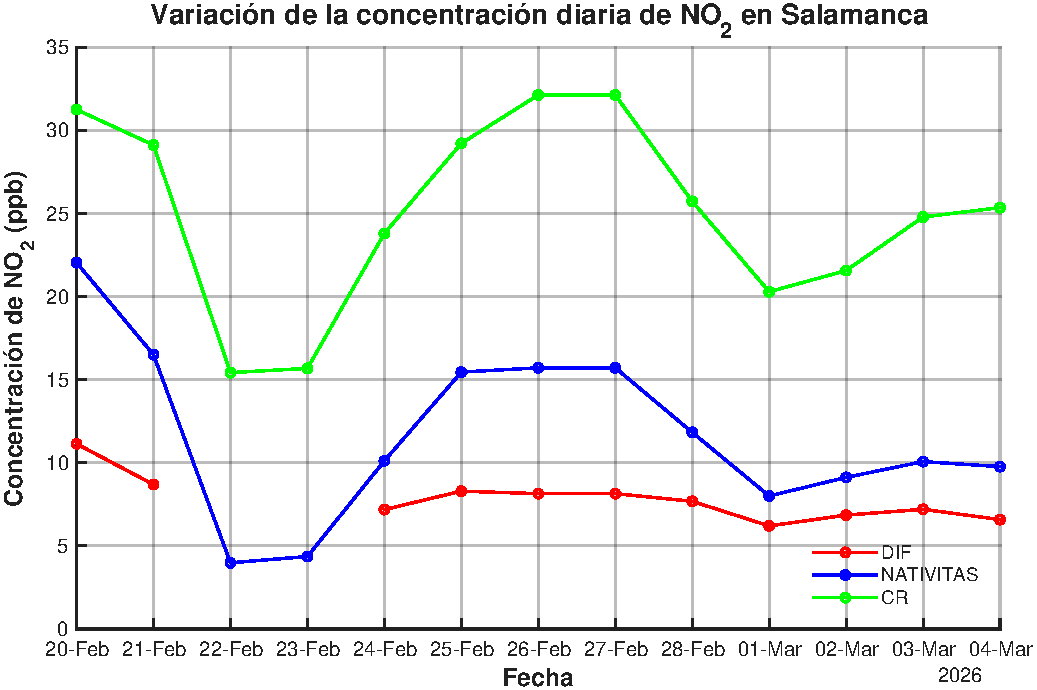
\includegraphics[width=0.85\textwidth]{Resultados/NO2_diario.pdf}
    \caption{Variación de la concentración de NO\textsubscript{2} en las
    estaciones de monitoreo del del 20 de febrero al 5 de marzo del 2026}
    \label{fig:no2}
\end{figure}

\begin{figure}[htbp]
    \centering
    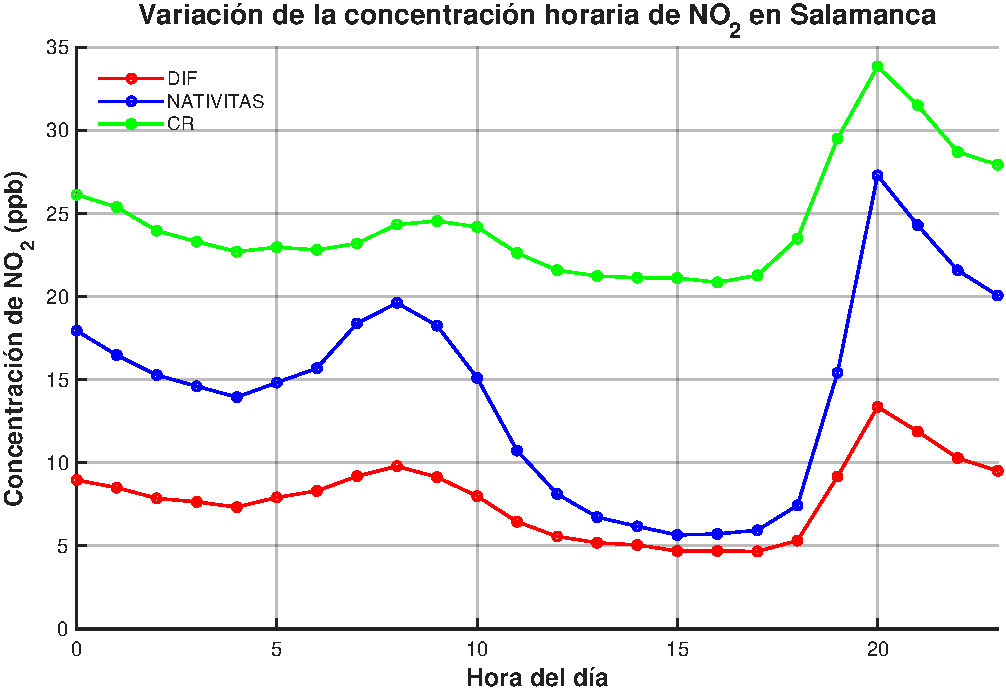
\includegraphics[width=0.85\textwidth]{Resultados/NO2_horario.pdf}
    \caption{Ciclo diurno de NO\textsubscript{2} en las estaciones de
    monitoreo del 20 de febrero al 5 de marzo del 2026}
    \label{fig:no2_horario}
\end{figure}

En la Figura~\ref{fig:rosa_estaciones} se presenta la rosa de los
vientos para las estaciones de Salamanca. Se observa un comportamiento
similar en los tres puntos, con vientos predominantes del sureste en un
rango de \SIrange{2.1}{3.6}{\meter\per\second}. Existen ligeras
variaciones en la frecuencia de vientos superiores a
\SI{3.6}{\meter\per\second}, los cuales tienden a ser más frecuentes en
la estación DIF.

Por otro lado, durante el periodo de muestreo los vientos predominantes
provienen del noreste. Los rangos más frecuentes son de
\SIrange{2.1}{3.6}{\meter\per\second} y de
\SIrange{3.6}{5.7}{\meter\per\second}. La dirección menos frecuente es
el noroeste, la cual solo aparece en vientos débiles de
\SIrange{0.5}{2.1}{\meter\per\second}
(Figura~\ref{fig:rosa_muestreo}).

\begin{figure}[htbp]
    \centering
    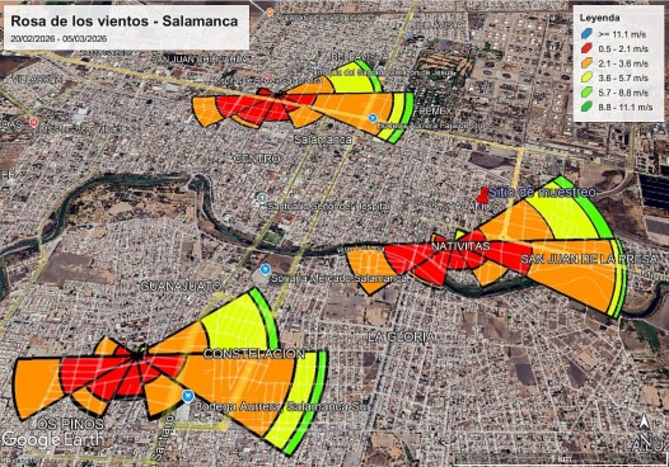
\includegraphics[width=0.85\textwidth]{Resultados/Rosa_diario.pdf}
    \caption{Rosas de los vientos de las estaciones de monitoreo de
    Salamanca.}
    \label{fig:rosa_estaciones}
\end{figure}

\begin{figure}[htbp]
    \centering
    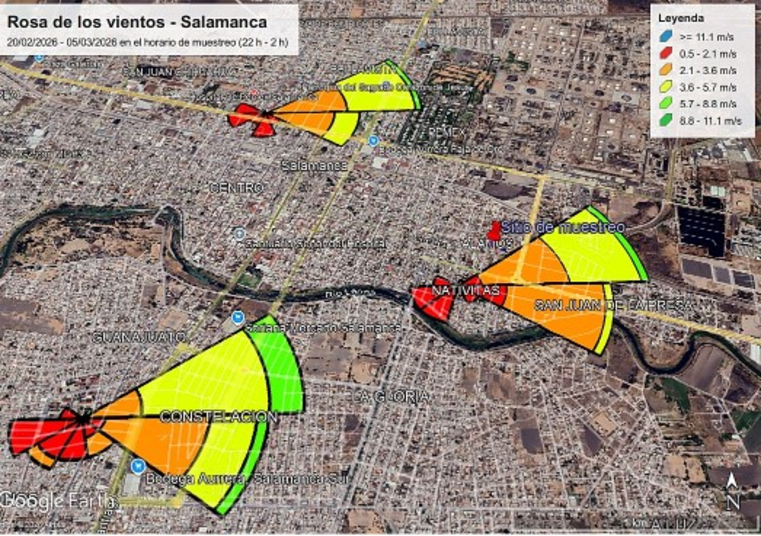
\includegraphics[width=0.6\textwidth]{Resultados/Rosa_horario.pdf}
    \caption{Rosa de los vientos durante el periodo de muestreo.}
    \label{fig:rosa_muestreo}
\end{figure}

\section{Composición isotópica}
La Figura~\ref{fig:mezcla_salamanca} presenta el diagrama
$\delta^{2}$H vs.\ $\delta^{18}$O construido para las muestras de vapor
de agua colectadas en el sitio Salamanca (puntos azules) y el extremo
composicional VDC (punto rojo), siguiendo el enfoque de mezcla de dos
componentes empleado por Xing et al.\ (2020). Los puntos de Salamanca se
agrupan en un rango relativamente estrecho, entre aproximadamente
$-6$\,\textperthousand\ y $-12$\,\textperthousand\ para
$\delta^{18}$O y entre $-75$\,\textperthousand\ y
$-120$\,\textperthousand\ para $\delta^{2}$H, mientras que el extremo
VDC se ubica en una posición claramente distinta, con valores de
$\delta^{18}\mathrm{O} \approx 9$\,\textperthousand\ y
$\delta^{2}\mathrm{H} \approx -135$\,\textperthousand.

Sobre este diagrama se trazaron dos líneas de referencia: la Línea
Meteórica Mundial (LMM), definida por la ecuación
$\delta^{2}\mathrm{H} = 8\,\delta^{18}\mathrm{O} + 10$, y la línea de
mezcla determinada por regresión para el sistema Salamanca--VDC
(LM-SDR), con ecuación
$\delta^{2}\mathrm{H} = 7.289\,\delta^{18}\mathrm{O} + 4.4899$, la cual
está dada por datos obtenidos en San Juan del Río, Querétaro. A partir
de estas dos líneas y del extremo VDC se construyeron isolíneas de
mezcla correspondientes a fracciones de 20, 40, 60 y 80\,\% de vapor de
combustión, siguiendo la ecuación de mezcla de dos componentes.

La distribución de los puntos de Salamanca respecto a estas isolíneas
muestra que la mayoría de las muestras se ubican entre las líneas
correspondientes a 20\,\% de mezcla, mientras que ninguna supera el
30\,\%. El punto VDC, por su posición en el extremo del triángulo de
mezcla, representa el 100\,\% del componente de vapor de combustión
considerado en el modelo.

\begin{figure}[htbp]
    \centering
    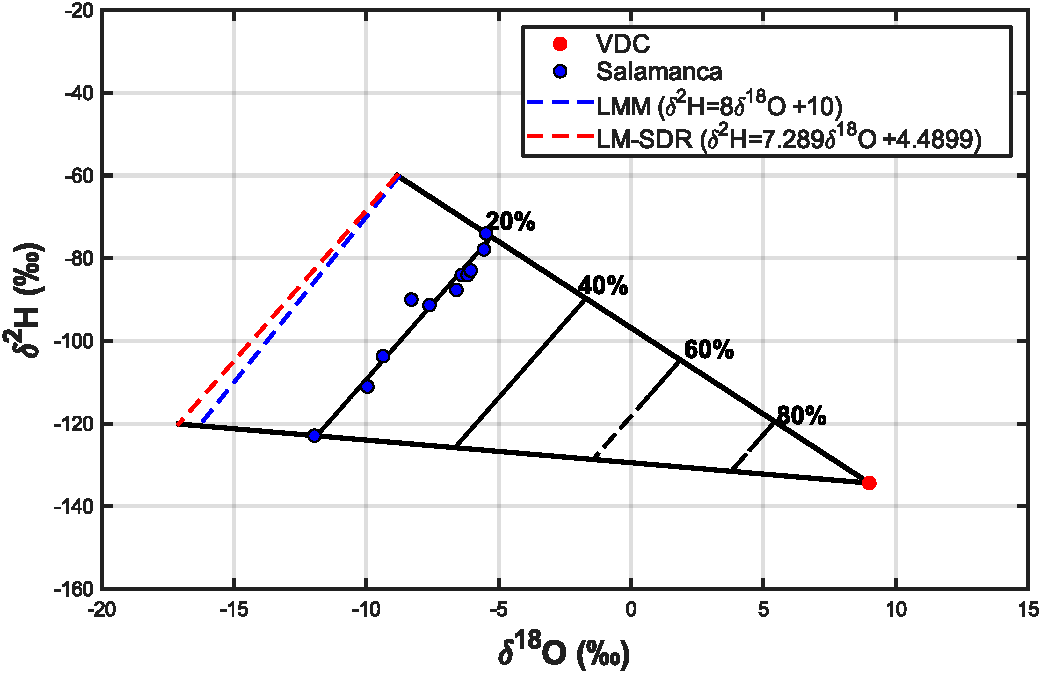
\includegraphics[width=0.8\textwidth]{Resultados/Mezcla_iso.pdf}
    \caption{Diagrama $\delta^{2}$H vs.\ $\delta^{18}$O del vapor de agua
    en Salamanca (puntos azules) y del extremo VDC (punto rojo), con la
    LMM, la LM-SDR e isolíneas de mezcla de 20, 40, 60 y 80\,\%.}
    \label{fig:mezcla_salamanca}
\end{figure}

\section{Modelo de dispersión FLEXPART}
La Figura~\ref{fig:retrotrayectorias} muestra la retrotrayectoria
promedio nocturna (22:00--02:00\,h), correspondiente al promedio de
todos los días de muestreo dentro de esta franja horaria, para los
cuatro sitios receptores considerados (Sitio de muestreo, Nativitas, DIF
y Cruz Roja).

El panel superior presenta el perfil vertical de la trayectoria,
expresado como altura sobre el nivel del suelo (km) en función de la
distancia horizontal a la estación (km). En él se observa que, en los
primeros $\sim$\SI{130}{\kilo\meter} previos a la llegada a los
receptores, las masas de aire de los cuatro sitios descienden de manera
prácticamente coincidente desde alturas de
\SIrange{3.0}{3.5}{\kilo\meter} hasta aproximadamente
\SIrange{1.5}{2.0}{\kilo\meter}. A distancias mayores, las trayectorias
se dispersan verticalmente, alcanzando alturas de
\SIrange{2.5}{5.0}{\kilo\meter}, con el sitio Cruz Roja (verde)
mostrando la mayor variabilidad en este segmento.

El panel inferior presenta la proyección horizontal de las mismas
retrotrayectorias sobre un mapa de la región de estudio, con la posición
de cada estación receptora marcada mediante un asterisco y el contorno
de la cuenca delimitado con línea punteada. Las cuatro trayectorias
siguen un recorrido horizontal muy similar entre sí, con dirección
predominante desde el sur-suroeste hacia el norte-noreste,
extendiéndose hasta poco más de \SI{400}{\kilo\meter} de distancia
respecto a las estaciones. Esto indica un origen común de las masas de
aire nocturnas durante el periodo de muestreo, independientemente del
sitio receptor considerado.

%begin{figure}[htbp]
 %  \centering
  % 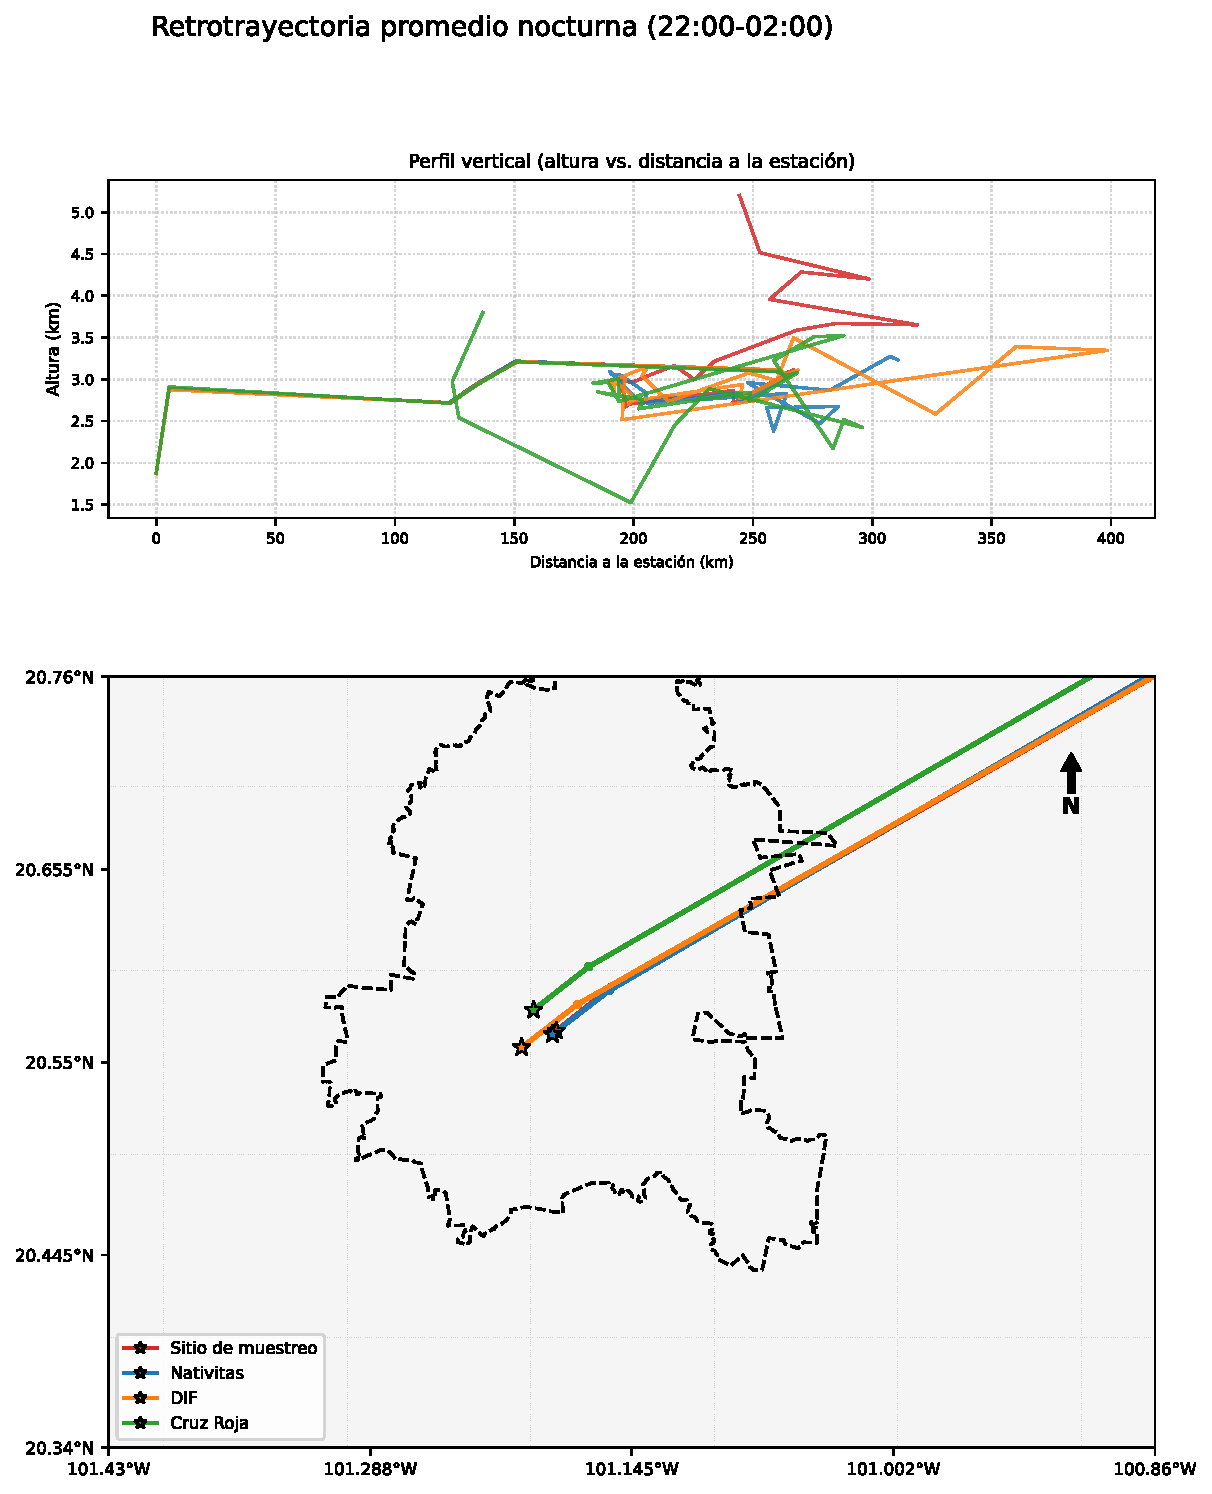
\includegraphics[width=0.85\textwidth]{Resultados/trayectoria_nocturna.pdf}
   %\caption{Retrotrayectoria promedio nocturna (22:00--02:00\,h) para
   %los sitios receptores. Panel superior: perfil vertical (altura sobre
  % el nivel del suelo vs.\ distancia horizontal). Panel inferior:
  % proyección horizontal sobre la región de estudio; los asteriscos
  % indican las estaciones receptoras y la línea punteada el contorno de
  % Salamanca.}
  % \label{fig:retrotrayectorias}
%end{figure}

La Figura~\ref{fig:retro_24h} presenta la retrotrayectoria promedio
calculada a partir de las 24\,h de cada día de muestreo, desagregada por
sitio receptor con un panel individual por estación. El panel superior
de cada columna muestra el perfil vertical de la trayectoria (altura
sobre el nivel del suelo, en km, en función de la distancia a la
estación, en km), mientras que el panel inferior presenta la proyección
horizontal correspondiente sobre el mapa de la región de estudio.

A diferencia del promedio restringido al horario nocturno
(22:00--02:00\,h), las trayectorias calculadas con el promedio de 24\,h
muestran un mayor grado de complejidad y variabilidad vertical en los
primeros \SIrange{200}{250}{\kilo\meter} previos a la llegada a cada
receptor. Las oscilaciones de altura alcanzan hasta
$\sim$\SI{1.5}{\kilo\meter} en Nativitas y DIF, y son de mayor amplitud
en Cruz Roja y Sitio de muestreo, donde se observan además tramos de
trayectoria con desplazamiento horizontal no monótono (retrocesos y
bucles) en la distancia recorrida. A distancias superiores a
$\sim$\SIrange{250}{300}{\kilo\meter}, las cuatro trayectorias adoptan
un comportamiento más suavizado, con un ascenso gradual de altura hacia
el origen de la retrotrayectoria, alcanzando valores máximos de entre
\SI{3.75}{\kilo\meter} (Nativitas y DIF) y \SI{5.0}{\kilo\meter} (Cruz
Roja y Sitio de muestreo).

En la proyección horizontal, los cuatro sitios muestran un patrón de
trayectoria consistente entre sí, con un recorrido predominante desde el
sur-suroeste hacia el norte-noreste de la estación receptora,
alcanzando distancias de entre \SI{300}{\kilo\meter} y
\SI{400}{\kilo\meter}. Esto sugiere un origen regional común de las
masas de aire durante el periodo de muestreo completo,
independientemente del sitio considerado.

%begin{figure}[htbp]
 %  \centering
 %  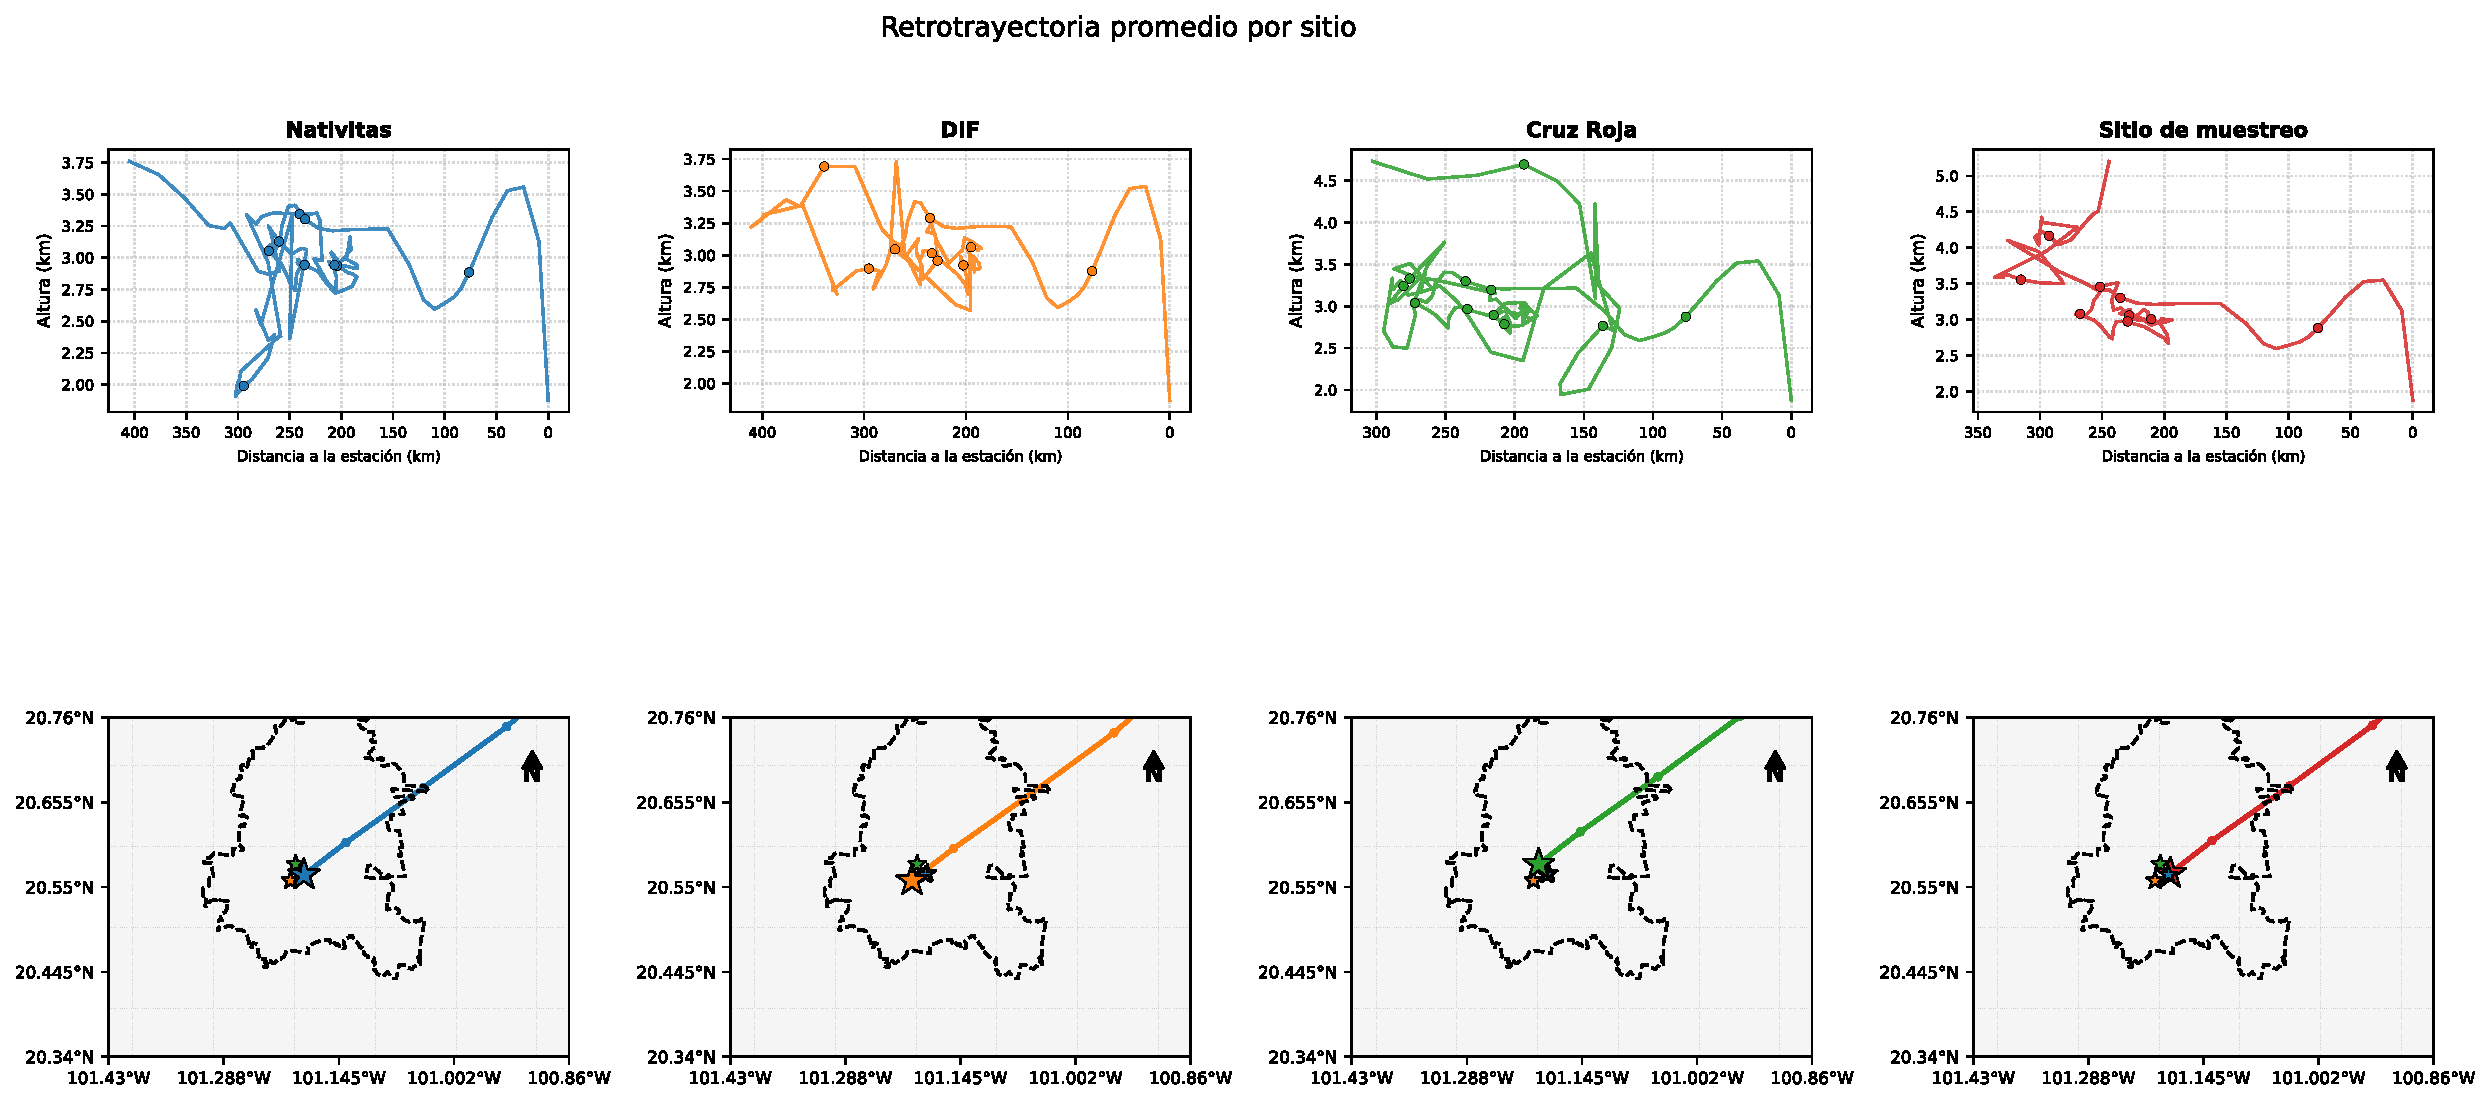
\includegraphics[width=\textwidth]{Resultados/trayectoria_diario.pdf}
 %  \caption{Retrotrayectoria promedio de 24\,h por sitio receptor
 %  (Sitio de muestreo, Nativitas, DIF y Cruz Roja). Panel superior:
 %  perfil vertical (altura sobre el nivel del suelo vs.\ distancia a la
 %  estación). Panel inferior: proyección horizontal sobre la región de
 %  estudio.}
 %  \label{fig:retro_24h}
%end{figure}

La Figura~\ref{fig:footprints_co} muestra las matrices de sensibilidad
fuente-receptor (\textit{footprints}) de CO obtenidas mediante las
simulaciones retro-trayectoria de FLEXPART para las cuatro estaciones de
monitoreo consideradas (Nativitas, DIF, Cruz Roja y Sitio de muestreo),
ubicadas en Salamanca, Guanajuato, durante el horario de muestreo
(22:00--02:00\,h).

En los cuatro paneles, los valores de sensibilidad más elevados
($>0.3$\,u.a., correspondientes a la porción verde-amarilla de la
escala) se concentran en una franja continua orientada hacia el sureste
del dominio modelado, en las inmediaciones directas de cada punto
receptor (marcado con un cuadro negro), y disminuyen de manera
progresiva conforme aumenta la distancia a la estación. Los valores
máximos de sensibilidad ($>0.5$\,u.a.) se registran en las celdas
contiguas a cada receptor. Fuera de esta franja, el resto del dominio
presenta valores de sensibilidad considerablemente menores, generalmente
inferiores a $0.1$\,u.a. (tonos azul y morado de la escala), abarcando
la mayor parte del área modelada.

El patrón espacial de la zona de mayor sensibilidad es similar entre las
cuatro estaciones, con diferencias menores en la extensión y orientación
exacta de la franja de alta sensibilidad, asociadas a la ubicación
particular de cada receptor dentro del dominio.

\begin{figure}[htbp]
    \centering
    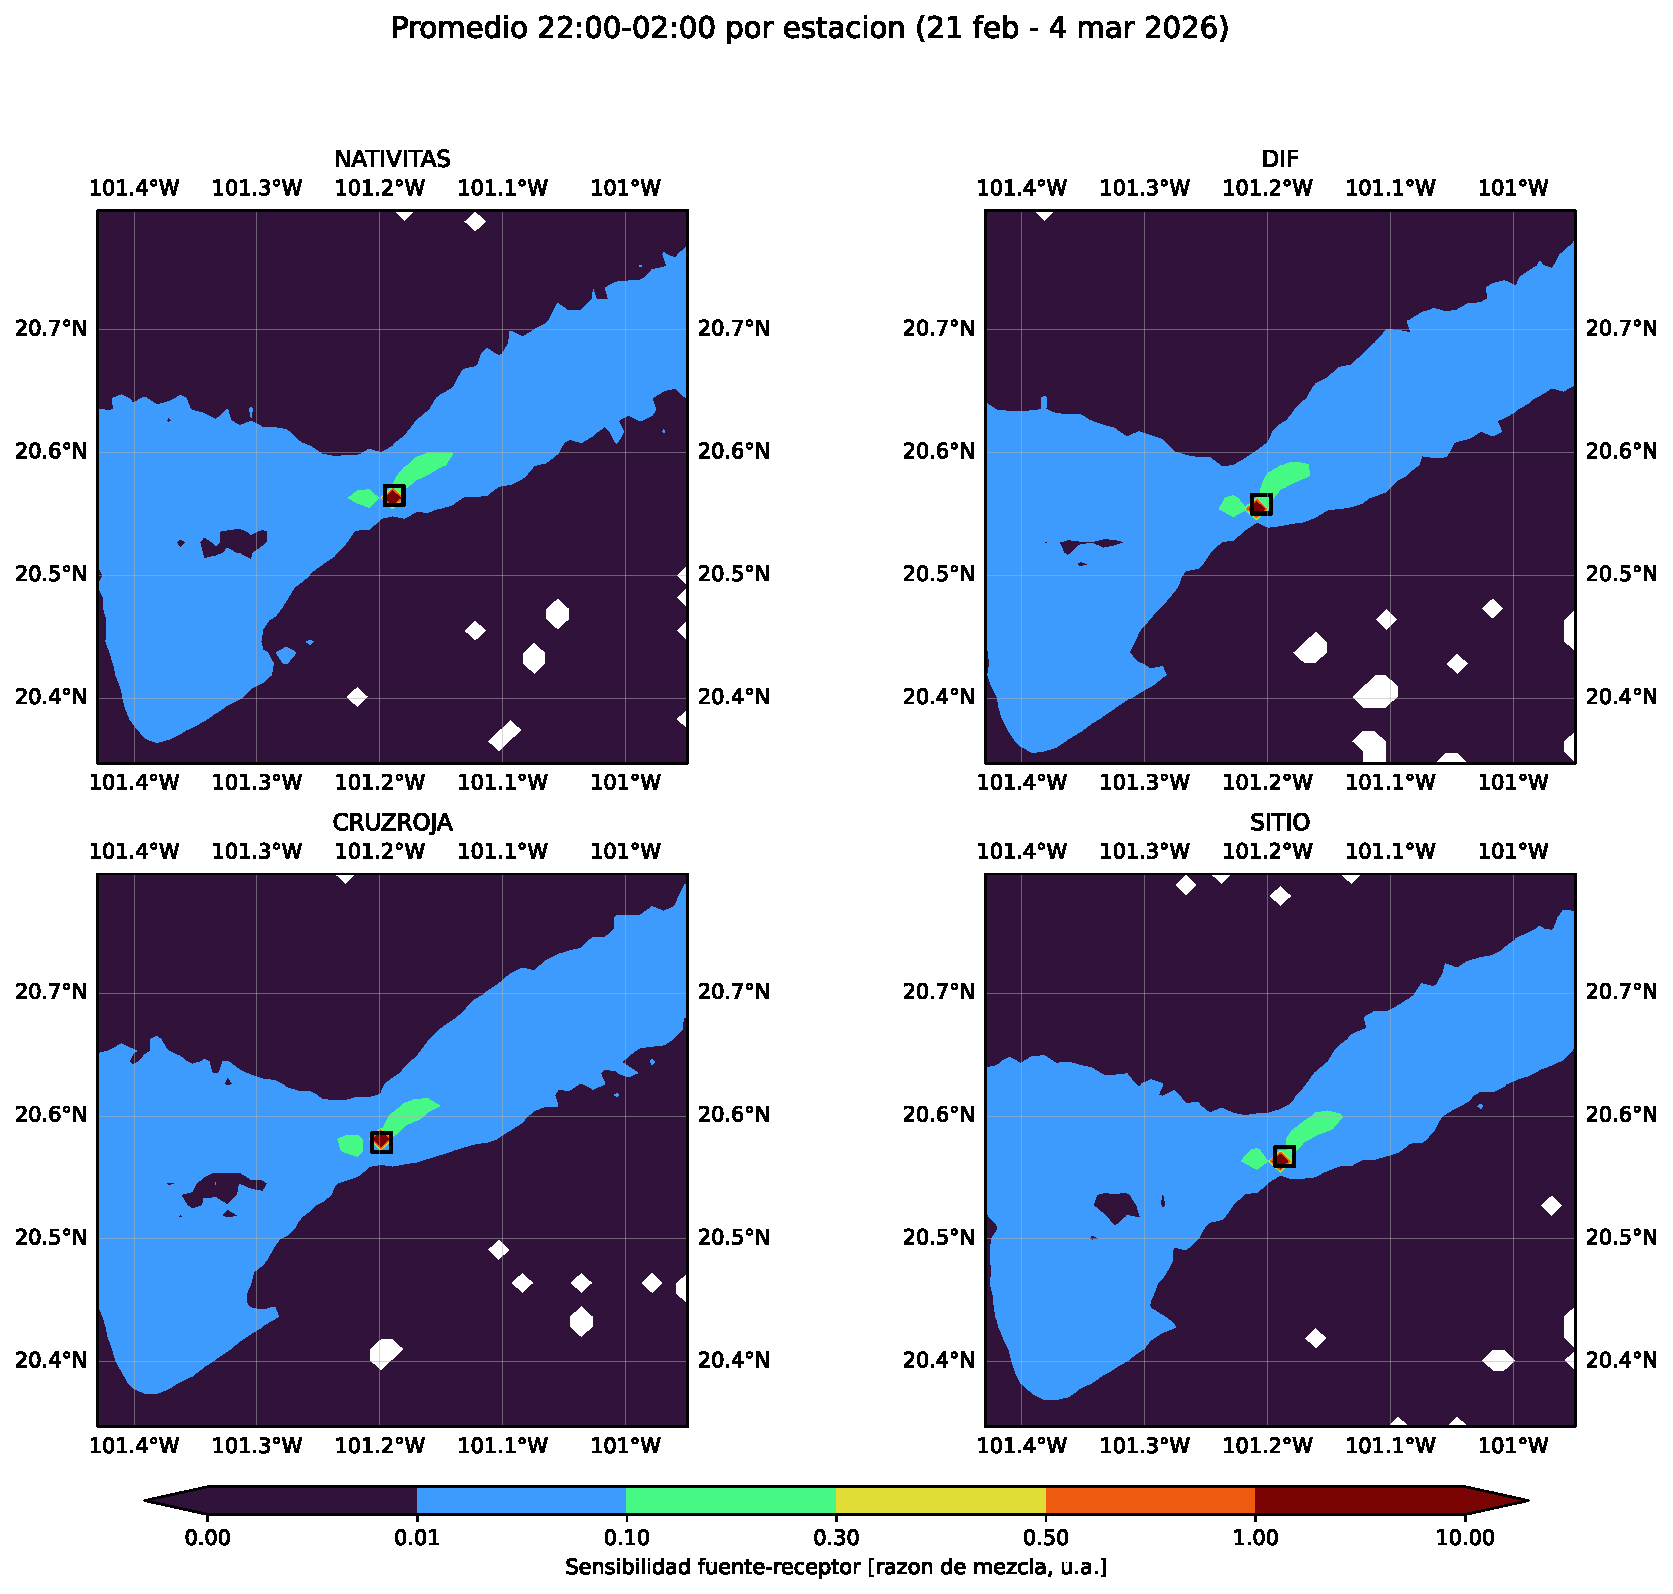
\includegraphics[width=\textwidth]{Resultados/FOOTPRINT_horario.pdf}
    \caption{Matrices de sensibilidad fuente-receptor (\textit{footprints})
    de CO obtenidas con FLEXPART en modo retro-trayectoria para las
    estaciones Nativitas, DIF, Cruz Roja y Sitio de muestreo, durante el
    horario de muestreo (22:00--02:00\,h). El cuadro negro indica la
    posición de cada receptor; la sensibilidad se expresa en unidades
    arbitrarias (u.a.).}
    \label{fig:footprints_co}
\end{figure}

La Figura~\ref{fig:footprints_co_24h} presenta las matrices de
sensibilidad fuente-receptor (\textit{footprints}) de CO
correspondientes al promedio de 24\,h durante todo el periodo de
muestreo, para las cuatro estaciones. Al igual que en el promedio
nocturno, los valores de sensibilidad más elevados ($>0.3$\,u.a.) se
concentran en una franja orientada hacia el sureste del dominio, en las
celdas inmediatas a cada punto receptor (marcado con un cuadro negro),
con los valores máximos ($>0.5$\,u.a.) restringidos a las celdas
contiguas al receptor.

Sin embargo, al considerar el ciclo diurno completo, esta zona de alta
sensibilidad se presenta de manera más compacta y de menor extensión
espacial en comparación con el promedio nocturno, lo que es consistente
con condiciones de mayor mezcla vertical y dispersión horizontal durante
las horas del día. El resto del dominio modelado mantiene valores de
sensibilidad bajos ($<0.1$\,u.a.), similares en magnitud y distribución
a los observados en el promedio nocturno.

El patrón espacial general es consistente entre las cuatro estaciones,
con variaciones menores en la orientación y extensión de la franja de
mayor sensibilidad, asociadas a la posición particular de cada receptor
dentro del dominio.

\begin{figure}[htbp]
    \centering
    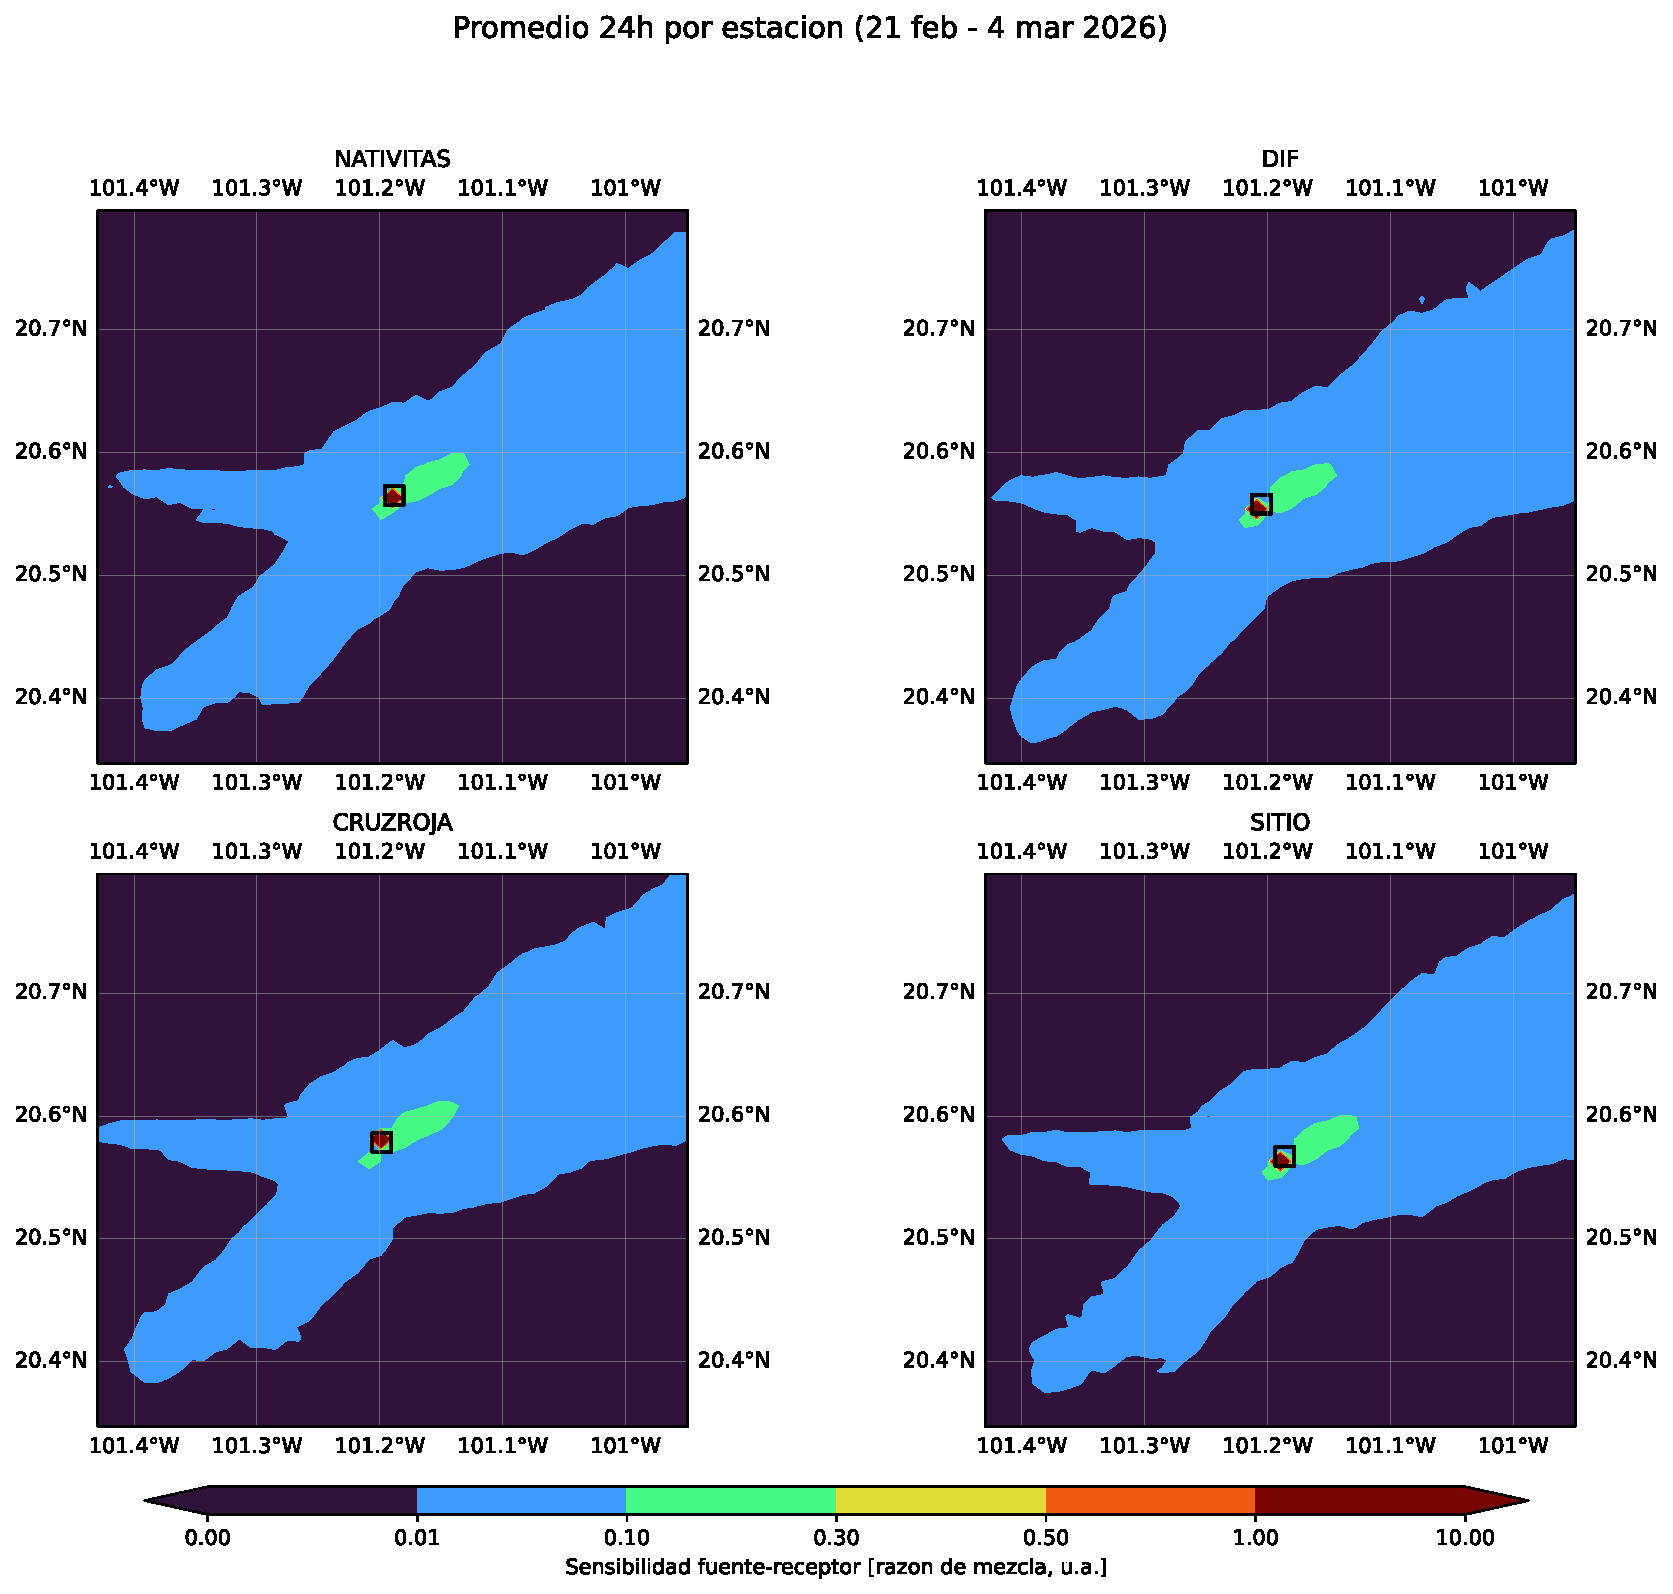
\includegraphics[width=\textwidth]{Resultados/FOOTPRINT_diario.pdf}
    \caption{Matrices de sensibilidad fuente-receptor (\textit{footprints})
    de CO obtenidas con FLEXPART para el promedio de 24\,h durante todo
    el periodo de muestreo, en las estaciones Nativitas, DIF, Cruz Roja y
    Sitio de muestreo. El cuadro negro indica la posición de cada
    receptor; la sensibilidad se expresa en unidades arbitrarias (u.a.).}
    \label{fig:footprints_co_24h}
\end{figure}